% !TEX program = pdflatex
\documentclass[tikz,border=5pt]{standalone}
\usepackage{tikz}
\usetikzlibrary{calc,arrows.meta,positioning,decorations.pathreplacing}

% ======= PARAMETERS ===================================
\newcommand{\PageW}{210}     % mm
\newcommand{\PageH}{297}     % mm
\newcommand{\InnerMargin}{28}
\newcommand{\BindingOffset}{8}
\newcommand{\OuterMargin}{48}
\newcommand{\TopMargin}{25}
\newcommand{\BottomMargin}{30}
\newcommand{\HeaderBand}{12}
\newcommand{\HeaderRuleGap}{5}
\newcommand{\FooterBand}{8}
\newcommand{\SidenoteWidth}{20}
% ======================================================

\begin{document}
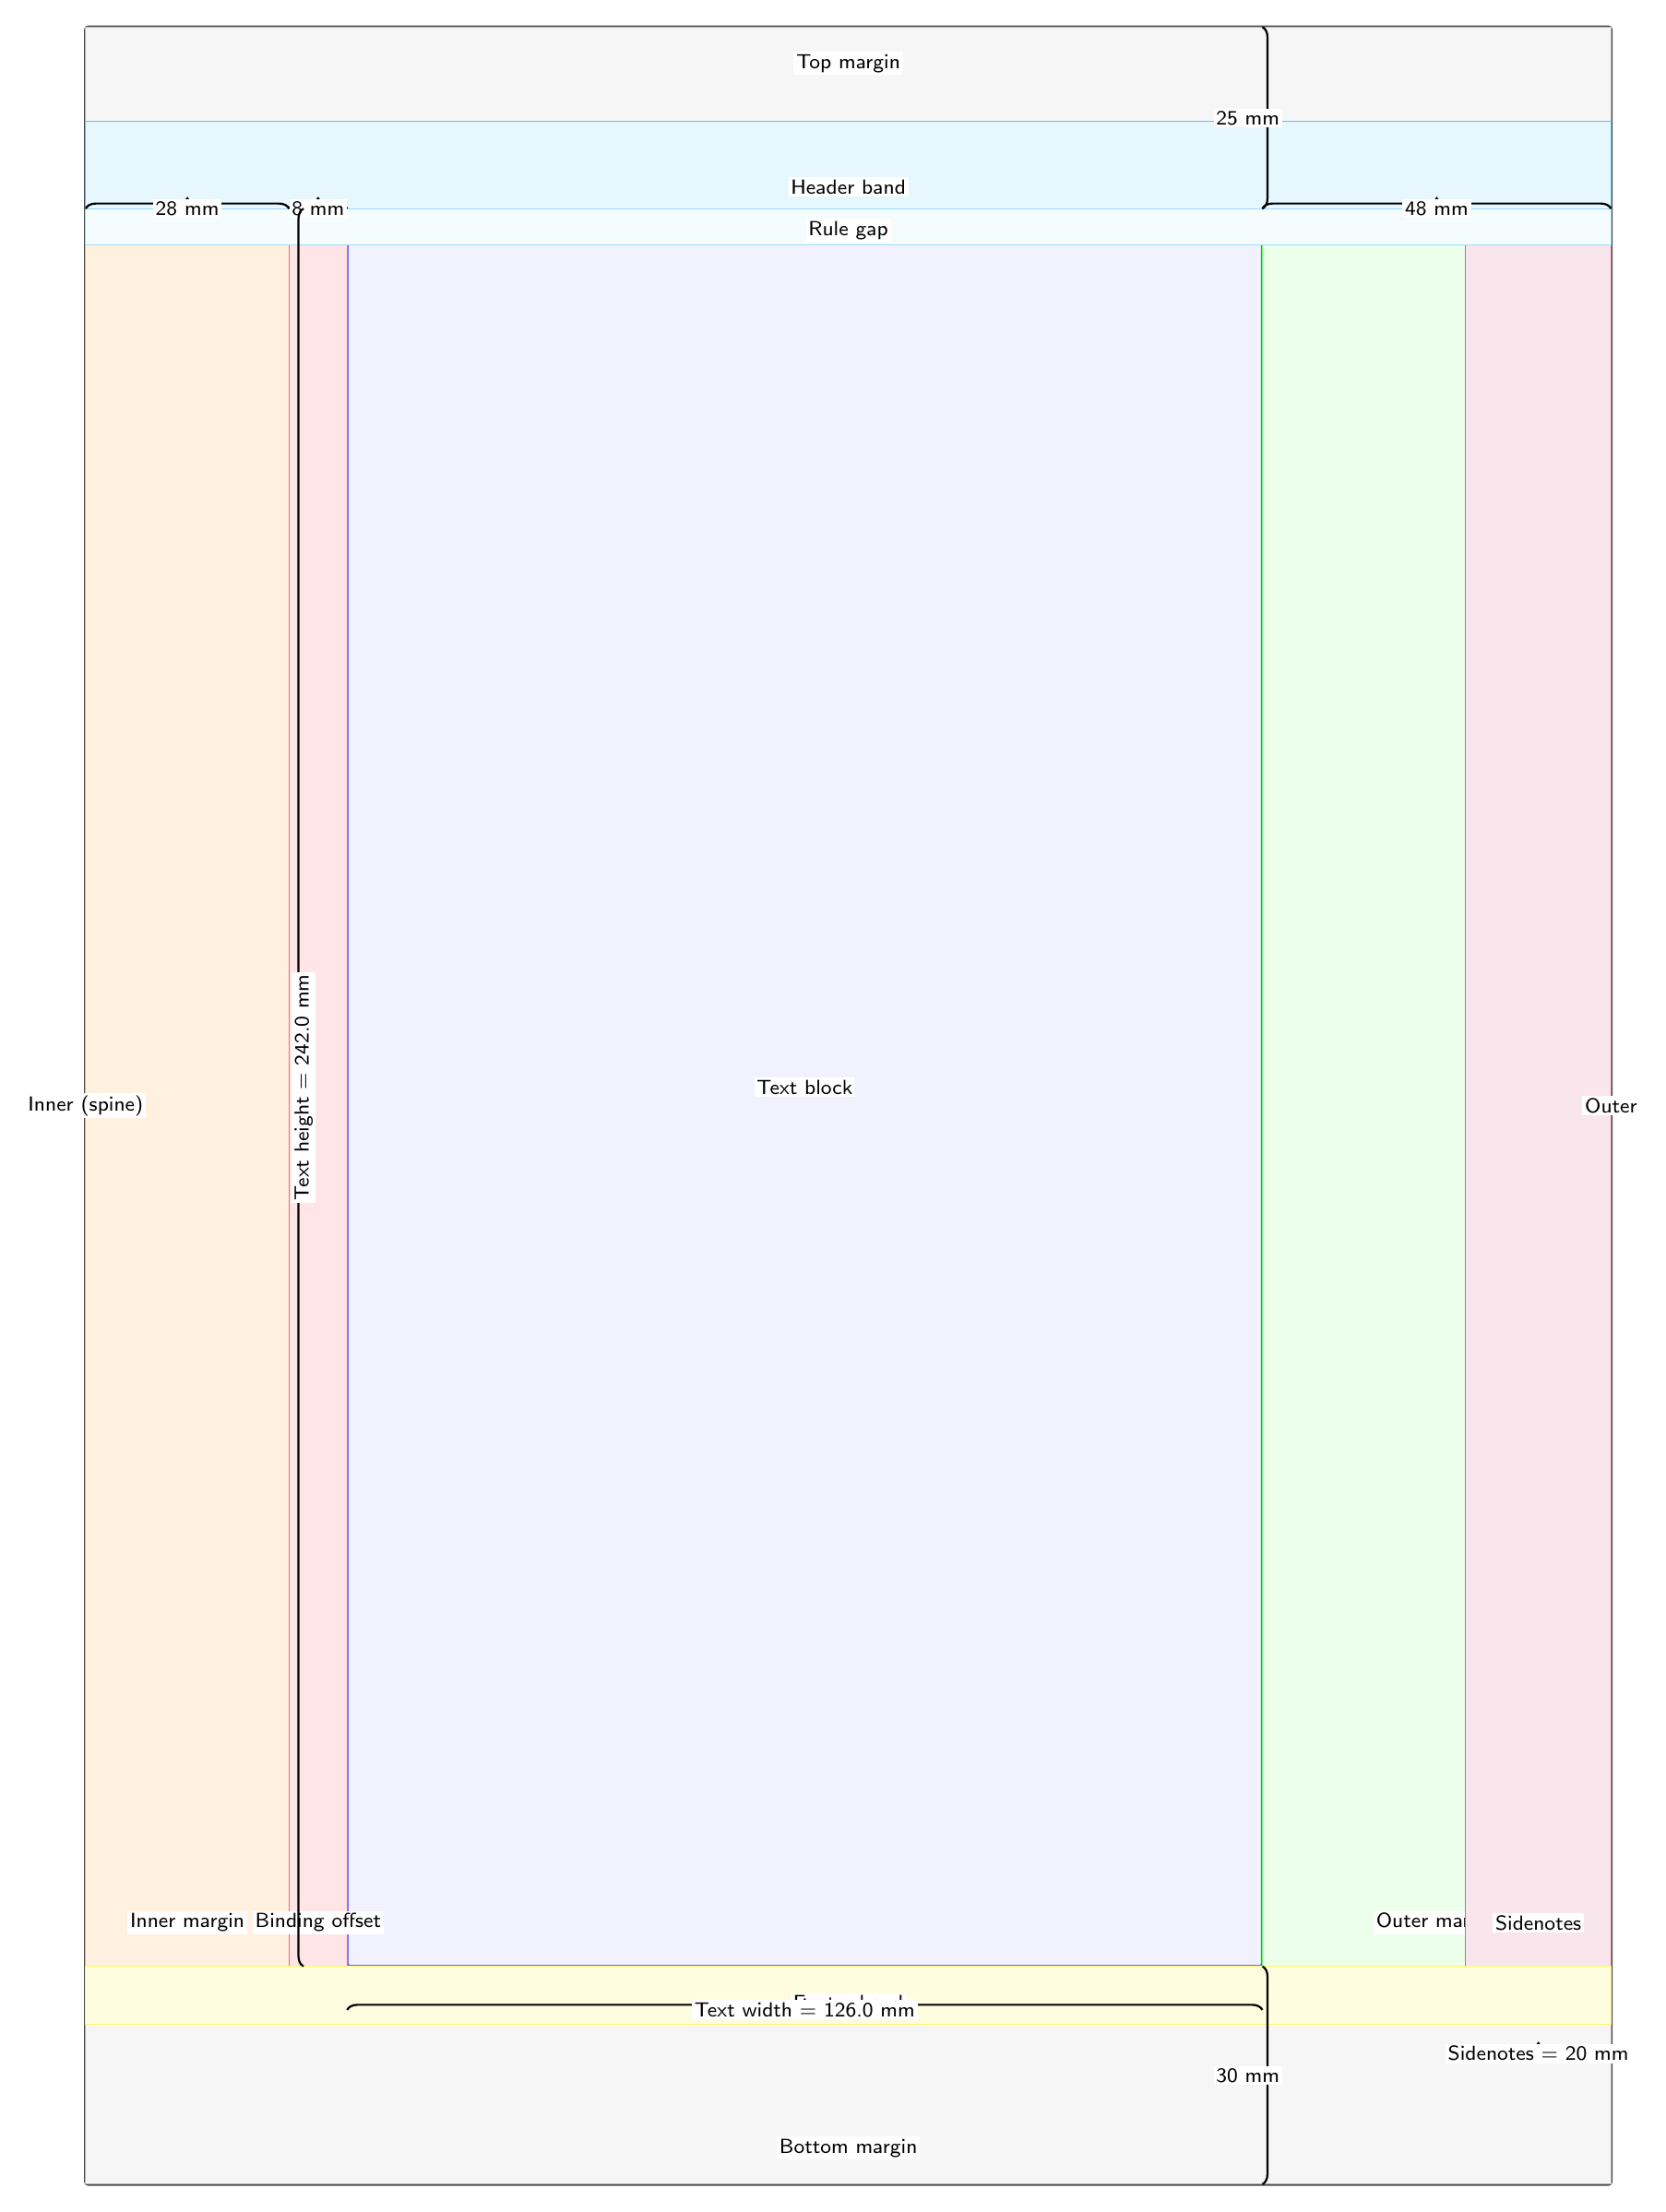
\begin{tikzpicture}[x=1mm,y=1mm,
  label/.style={font=\sffamily\footnotesize, fill=white, inner sep=1pt},
  brace/.style={decorate, decoration={brace, amplitude=4pt}, thick},
  mline/.style={very thick, rounded corners=1pt},
  annot/.style={-Latex, thick}
]

% ----- Derived values -----
\pgfmathsetmacro{\InnerEdge}{0}
\pgfmathsetmacro{\OuterEdge}{\PageW}
\pgfmathsetmacro{\InnerWithBind}{\InnerMargin + \BindingOffset}
\pgfmathsetmacro{\TextXmin}{\InnerWithBind}
\pgfmathsetmacro{\TextXmax}{\PageW - \OuterMargin}
\pgfmathsetmacro{\TextYmin}{\BottomMargin}
\pgfmathsetmacro{\TextYmax}{\PageH - \TopMargin}
\pgfmathsetmacro{\TextWidth}{\PageW - \OuterMargin - (\InnerMargin + \BindingOffset)}
\pgfmathsetmacro{\TextHeight}{\PageH - \TopMargin - \BottomMargin}
\pgfmathsetmacro{\SidenoteXmin}{\OuterEdge - \SidenoteWidth}
\pgfmathsetmacro{\HeaderBottom}{\PageH - \TopMargin}
\pgfmathsetmacro{\HeaderTop}{\HeaderBottom + \HeaderBand}
\pgfmathsetmacro{\RuleGapTop}{\HeaderBottom}
\pgfmathsetmacro{\RuleGapBottom}{\HeaderBottom - \HeaderRuleGap}
\pgfmathsetmacro{\FooterTop}{\BottomMargin}
\pgfmathsetmacro{\FooterBottom}{\BottomMargin - \FooterBand}

% Page rectangle
\draw[mline, black!70] (0,0) rectangle (\PageW,\PageH);

% Text block
\fill[blue!5] (\TextXmin,\TextYmin) rectangle (\TextXmax,\TextYmax);
\draw[mline, blue!60] (\TextXmin,\TextYmin) rectangle (\TextXmax,\TextYmax);
\node[label] at ($(\TextXmin,\TextYmin)!0.5!(\TextXmax,\TextYmax)$) {Text block};

% Inner margin (without binding)
\fill[orange!12] (\InnerEdge, \TextYmin) rectangle (\InnerMargin, \TextYmax);
\draw[orange!60] (\InnerEdge, \TextYmin) rectangle (\InnerMargin, \TextYmax);
\node[label] at ($(\InnerEdge,\TextYmin+6)!0.5!(\InnerMargin,\TextYmin+6)$) {Inner margin};

% Binding offset band
\fill[red!10] (\InnerMargin, \TextYmin) rectangle (\InnerWithBind, \TextYmax);
\draw[red!60] (\InnerMargin, \TextYmin) rectangle (\InnerWithBind, \TextYmax);
\node[label] at ($(\InnerMargin,\TextYmin+6)!0.5!(\InnerWithBind,\TextYmin+6)$) {Binding offset};

% Outer margin band
\fill[green!8] (\TextXmax, \TextYmin) rectangle (\OuterEdge, \TextYmax);
\draw[green!60] (\TextXmax, \TextYmin) rectangle (\OuterEdge, \TextYmax);
\node[label] at ($(\TextXmax,\TextYmin+6)!0.5!(\OuterEdge,\TextYmin+6)$) {Outer margin};

% Sidenote area
\fill[purple!10] (\SidenoteXmin, \TextYmin) rectangle (\OuterEdge, \TextYmax);
\draw[purple!60] (\SidenoteXmin, \TextYmin) rectangle (\OuterEdge, \TextYmax);
\node[label] at ($(\SidenoteXmin,\TextYmin+6)!0.5!(\OuterEdge,\TextYmin+6)$) {Sidenotes};

% Top & bottom margin bands
\fill[gray!7] (\InnerEdge, \TextYmax) rectangle (\OuterEdge, \PageH);
\draw[gray!60] (\InnerEdge, \TextYmax) rectangle (\OuterEdge, \PageH);
\node[label] at (\PageW/2, \PageH - 5) {Top margin};

\fill[gray!7] (\InnerEdge, 0) rectangle (\OuterEdge, \TextYmin);
\draw[gray!60] (\InnerEdge, 0) rectangle (\OuterEdge, \TextYmin);
\node[label] at (\PageW/2, 5) {Bottom margin};

% Header band + rule gap
\fill[cyan!10] (\InnerEdge, \HeaderBottom) rectangle (\OuterEdge, \HeaderTop);
\draw[cyan!70] (\InnerEdge, \HeaderBottom) rectangle (\OuterEdge, \HeaderTop);
\node[label] at (\PageW/2, \HeaderBottom + 3) {Header band};

\fill[cyan!4] (\InnerEdge, \RuleGapBottom) rectangle (\OuterEdge, \RuleGapTop);
\draw[cyan!40] (\InnerEdge, \RuleGapBottom) rectangle (\OuterEdge, \RuleGapTop);
\node[label] at (\PageW/2, \RuleGapBottom + 2) {Rule gap};

% Footer band
\fill[yellow!12] (\InnerEdge, \FooterBottom) rectangle (\OuterEdge, \FooterTop);
\draw[yellow!60] (\InnerEdge, \FooterBottom) rectangle (\OuterEdge, \FooterTop);
\node[label] at (\PageW/2, \FooterBottom + 3) {Footer band};

% ===== Dimension Braces =====
\draw[brace] ([xshift=0mm]0,\TextYmax) -- node[label] {\InnerMargin\ mm} ([xshift=0mm]\InnerMargin,\TextYmax);
\draw[brace] ([xshift=0mm]\InnerMargin,\TextYmax) -- node[label] {\BindingOffset\ mm} ([xshift=0mm]\InnerWithBind,\TextYmax);
\draw[brace] ([xshift=0mm]\TextXmax,\TextYmax) -- node[label] {\OuterMargin\ mm} ([xshift=0mm]\PageW,\TextYmax);

\draw[brace] (\TextXmax, \PageH) -- node[label, xshift=-2mm] {\TopMargin\ mm} (\TextXmax, \TextYmax);
\draw[brace] (\TextXmax, \TextYmin) -- node[label, xshift=-2mm] {\BottomMargin\ mm} (\TextXmax, 0);

\draw[brace] (\TextXmin, \TextYmin-6) -- node[label] {Text width = \TextWidth\ mm} (\TextXmax, \TextYmin-6);
\draw[brace] (\TextXmin-6, \TextYmin) -- node[label, rotate=90] {Text height = \TextHeight\ mm} (\TextXmin-6, \TextYmax);

\draw[brace] (\SidenoteXmin, \TextYmin-12) -- node[label] {Sidenotes = \SidenoteWidth\ mm} (\OuterEdge, \TextYmin-12);

\node[label] at (0, \PageH/2) {Inner (spine)};
\node[label] at (\PageW, \PageH/2) {Outer};

\end{tikzpicture}
\end{document}
